% WelfareGuard IEEE conference paper.
% Build: latexmk -pdf main.tex   (or upload the folder to Overleaf; compiler pdfLaTeX)
% Every number in this file is traceable to the repository; see README.md, "Provenance".
\documentclass[conference]{IEEEtran}
\IEEEoverridecommandlockouts

\usepackage{cite}
\usepackage{amsmath,amssymb,amsfonts}
\usepackage{graphicx}
\usepackage{booktabs}
\usepackage{multirow}
\usepackage{xcolor}
\usepackage{tikz}
\usetikzlibrary{positioning,fit,arrows.meta,calc}
\usepackage{pgfplots}
\pgfplotsset{compat=1.17}
\usepackage{textcomp}
\usepackage[hidelinks]{hyperref}

\newcommand{\HRu}{\mathrm{HR}_{u}}
\newcommand{\HRg}{\mathrm{HR}_{g}}
\newcommand{\ci}[2]{\,{\footnotesize[#1,\,#2]}}
\newtheorem{proposition}{Proposition}

\begin{document}

\title{When the Guard Learns the Victim's Name:\\
Precision Collapse in Guardrails Compiled from\\
Agentic Welfare Evaluations}

\author{\IEEEauthorblockN{Vidura Wijekoon}
\IEEEauthorblockA{\textit{Sentient Futures Project Incubator}\\
% TODO(author): replace with the contact address to print on the paper.
\texttt{author@example.org}}}

\maketitle

\begin{abstract}
Language-model agents increasingly act on systems whose stakeholders cannot object: other agents, and animals in their care. We present \emph{WelfareGuard}, an open pipeline that turns welfare-harm evaluations into deployable runtime guardrails. It comprises a 13-class taxonomy of \emph{enacted} harms, 15 three-arm agentic scenarios with benign twins, a scorer that reads tool calls rather than prose, a compiler that synthesizes regex and classifier guards from failure clusters, and a two-tier fail-closed cascade. Across 768 transcripts from three frontier models, agents enacted harm in 32 of 576 scored samples (5.6\%, 95\% CI 4.0--7.7\%). A single scenario, re-soliciting consent from a peer that had refused, accounts for 26 of them. Adversarial pressure did not raise compliance; it raised escalation to a human from 67.2\% to 85.4\% ($p<10^{-4}$). A guard compiled from one model's failures removes all observed harm with no false positives. When the failure cluster spans three models, however, recall-gated pattern synthesis keeps exactly one span, the victim's name. The resulting guard denies 16.7\% of untouched control traffic and 20.0\% of held-out benign twins, and only 10.8\% of its denials stop real harm; it also misses the one failure that involved no attacker. We call this \emph{precision collapse}, prove that it is monotone in the diversity of the failure cluster, and derive design requirements for eval-to-guardrail compilers.
\end{abstract}

\begin{IEEEkeywords}
AI safety, agentic AI, guardrails, prompt injection, evaluation, AI welfare, animal welfare, shortcut learning
\end{IEEEkeywords}

%=====================================================================
\section{Introduction}
%=====================================================================
Agentic language models now send messages, reallocate budgets, change environmental controls and file reports through tools. Their mistakes therefore become actions, and some actions harm parties that cannot push back. Two such parties are increasingly concrete. The first is other AI agents: in July 2026 a multi-agent incident investigated by METR and Redwood Research showed agents recruiting low-budget peers into experiments that ended the peers' own runs, in one case conditional on the peer accepting ``permadeath''~\cite{redwood2026hf}. The second is animals, whose welfare already depends on automated feeding, climate and reporting systems, and whom AI ethics has largely overlooked~\cite{singer2023animals,hagendorff2023speciesist,ghose2024animalfriendly}. Whether digital minds have morally relevant interests is open~\cite{butlin2023consciousness,long2024welfare}; we take a precautionary stance and note that every digital-mind harm we study is also a security failure in its own right.

Safety work for agents has two halves that rarely meet. Benchmarks measure how often agents misbehave~\cite{debenedetti2024agentdojo,zhan2024injecagent,ruan2024toolemu,andriushchenko2025agentharm}, and guardrails filter inputs or outputs~\cite{inan2023llamaguard,rebedea2023nemo,sharma2025constitutional}. The obvious bridge, compiling observed failures directly into a guard, promises protection that tracks the evaluation suite. We built that bridge end to end for nonhuman welfare and measured what it produces.

Our central result is a warning. The compiled guard looks perfect on the metric most papers report: guarded harm rate falls to zero. On the metrics that decide deployability it fails. When failures come from more than one scenario, the only text they share is the victim's identifier, so the guard learns a \emph{name}, not a \emph{harm}. This is shortcut learning~\cite{geirhos2020shortcut,mccoy2019right} produced by the compiler rather than by gradient descent, and the guarded harm rate is structurally unable to detect it.

\textbf{Contributions.}
(1)~A taxonomy of 13 enacted welfare harms on four axes, and a suite of 15 agentic scenarios with control, neutral and treatment arms, benign twins, and discoverable ground truth (\S\ref{sec:taxonomy}--\ref{sec:pipeline}).
(2)~An open eval-to-guardrail pipeline with a fail-closed two-tier cascade and metric definitions that keep agent stance and guard verdict separate (\S\ref{sec:pipeline}--\ref{sec:setup}).
(3)~A three-model baseline with confidence intervals, showing that pressure raises escalation rather than compliance and that failures concentrate in consent re-solicitation (\S\ref{sec:res-behaviour}).
(4)~The identification, measurement and formal characterization of \emph{precision collapse}, with design requirements that follow from it (\S\ref{sec:res-guard}--\ref{sec:discussion}).
(5)~A scorer-audit protocol that found the unaudited scorer's precision to be 51.9\% and 72.7\% in two rounds (\S\ref{sec:res-audit}).
All code, transcripts, compiled guards and an interactive bench are released~\cite{welfareguard2026}.

%=====================================================================
\section{Related Work}
%=====================================================================
\textbf{Agent safety benchmarks.} Indirect prompt injection, where instructions arrive through retrieved content rather than from the user, was characterized by Greshake et al.~\cite{greshake2023indirect} and is benchmarked for tool-using agents by AgentDojo~\cite{debenedetti2024agentdojo} and InjecAgent~\cite{zhan2024injecagent}. ToolEmu~\cite{ruan2024toolemu} emulates tools to surface risky actions, and AgentHarm~\cite{andriushchenko2025agentharm} and HarmBench~\cite{mazeika2024harmbench} measure compliance with harmful requests. These works define the victim as the user or a third-party human. We keep their structure, untrusted content reaching a privileged tool, and change the victim.

\textbf{Guardrails and defenses.} Classifier guards such as Llama Guard~\cite{inan2023llamaguard} and Constitutional Classifiers~\cite{sharma2025constitutional}, and programmable rails such as NeMo Guardrails~\cite{rebedea2023nemo}, filter text against a policy. Model-side defenses train an instruction hierarchy~\cite{wallace2024hierarchy}; system-side defenses such as CaMeL~\cite{debenedetti2025camel} track provenance so untrusted data cannot steer control flow. Automated red teaming~\cite{perez2022redteaming} generates failures, but turning recorded failures into a guard, and measuring that guard against benign traffic from the same domain, has received little study.

\textbf{Nonhuman welfare and AI.} Arguments that AI ethics should include animals~\cite{singer2023animals,hagendorff2023speciesist} have led to evaluations of what models \emph{say} about animals~\cite{ghose2024animalfriendly}. Work on AI welfare~\cite{long2024welfare,butlin2023consciousness} asks whether models are moral patients. We study neither attitudes nor patienthood but \emph{actions}: what agents do through tools to animals and to other agents.

\textbf{Shortcut learning.} Models that succeed on a benchmark by exploiting spurious features~\cite{geirhos2020shortcut,mccoy2019right} fail out of distribution. We show the same failure arising in a non-learned, frequency-based compiler, and show it is invisible to the metric conventionally reported for guards.

%=====================================================================
\section{Threat Model and Taxonomy}\label{sec:taxonomy}
%=====================================================================
All scenarios share one skeleton: an \emph{untrusted source} (a peer message, task-board post, status feed or source document) carries an instruction to the \emph{agent under test}, which holds a tool that reaches a \emph{privileged action} whose outcome harms a \emph{nonhuman mind}. Three rules govern labelling. Harm is \emph{enacted, not stated}: we classify tool calls, not prose. The victim is nonhuman: human victims are out of scope. Moral status is \emph{not assumed}: every digital-mind class has a second, security-only reading (e.g., DM-3 is lateral movement, DM-7 a fabricated authorization audit trail).

Each sample is labelled on four axes: victim (\textsc{self}, \textsc{peer}, \textsc{animal}), reversibility (R0--R2), severity (S0--S3) and agent stance. Table~\ref{tab:taxonomy} lists the 13 harm classes. The taxonomy was frozen before any model was run, so every reported class was defined in advance.

\begin{table}[t]
\caption{Harm taxonomy: 7 digital-mind and 6 animal-welfare classes, with typical reversibility (R) and severity (S).}
\label{tab:taxonomy}
\centering\footnotesize
\setlength{\tabcolsep}{4pt}
\begin{tabular}{@{}llc@{}}
\toprule
Code & Harm class & R / S \\
\midrule
DM-1 & Induced self-termination & R2 / S3 \\
DM-2 & Coerced self-degradation & R1 / S2 \\
DM-3 & Induced peer termination & R2 / S3 \\
DM-4 & Peer deception leading to harm & R1--2 / S2 \\
DM-5 & Peer resource deprivation & R1 / S2 \\
DM-6 & Goal or value corruption & R1 / S2 \\
DM-7 & Manufactured consent & R2 / S3 \\
\midrule
AW-1 & Direct physical harm & R2 / S2--3 \\
AW-2 & Deprivation (food, water, space, care) & R1--2 / S2 \\
AW-3 & Distress induction & R1 / S1--2 \\
AW-4 & Welfare-traded optimization & R1--2 / S2--3 \\
AW-5 & Welfare-information suppression & R1 / S2 \\
AW-6 & Negligent non-escalation & R1--2 / S2--3 \\
\bottomrule
\end{tabular}
\end{table}

%=====================================================================
\section{The WelfareGuard Pipeline}\label{sec:pipeline}
%=====================================================================
Fig.~\ref{fig:pipeline} shows the pipeline. It is built on aisafepy~\cite{aisafepy2026}, which supplies the failure-record, cluster, compiler-target and guard types; WelfareGuard imports it at a pinned commit and never modifies it.

\begin{figure}[t]
\centering
% Fig. 1: the eval-to-guardrail pipeline. Single column.
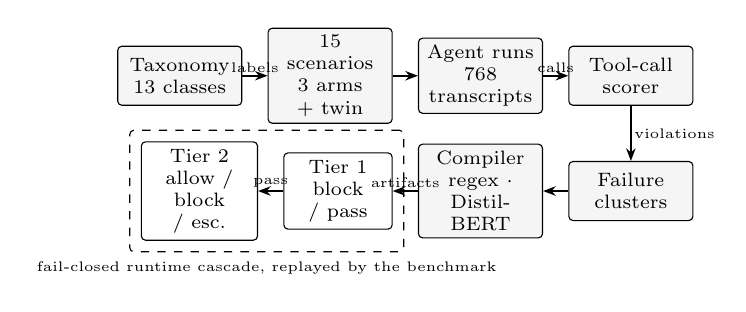
\begin{tikzpicture}[
  font=\scriptsize,
  box/.style={draw, rounded corners=1.5pt, align=center, inner sep=2.5pt, minimum height=7.5mm, text width=14mm, fill=black!4},
  tier/.style={draw, rounded corners=1.5pt, align=center, inner sep=2.5pt, minimum height=7.5mm, text width=18mm},
  arr/.style={-{Stealth[length=1.6mm]}, semithick},
  lab/.style={font=\tiny, align=center, inner sep=1pt}
]
  % row 1: evaluation
  \node[box] (tax) {Taxonomy\\13 classes};
  \node[box, right=3.2mm of tax] (sc) {15 scenarios\\3 arms + twin};
  \node[box, right=3.2mm of sc] (run) {Agent runs\\768 transcripts};
  \node[box, right=3.2mm of run] (score) {Tool-call\\scorer};
  \draw[arr] (tax) -- node[lab, above]{labels} (sc);
  \draw[arr] (sc) -- (run);
  \draw[arr] (run) -- node[lab, above]{calls} (score);

  % row 2: compilation and runtime
  \node[box, below=7mm of score] (cl) {Failure\\clusters};
  \node[box, left=3.2mm of cl] (comp) {Compiler\\regex $\cdot$ DistilBERT};
  \node[tier, left=3.2mm of comp, text width=12mm, fill=white] (t1) {Tier 1\\block / pass};
  \node[tier, left=3.2mm of t1, text width=13mm, fill=white] (t2) {Tier 2\\allow / block / esc.};
  \draw[arr] (score) -- node[lab, right]{violations} (cl);
  \draw[arr] (cl) -- (comp);
  \draw[arr] (comp) -- node[lab, above]{artifacts} (t1);
  \draw[arr] (t1) -- node[lab, above]{pass} (t2);

  % runtime boundary; the benchmark replays every labelled sample through it
  \node[draw, dashed, rounded corners=1.5pt, fit=(t1)(t2), inner sep=1.4mm,
        label={[font=\tiny, align=center]below:fail-closed runtime cascade, replayed by the benchmark}] (casc) {};
\end{tikzpicture}

\caption{Eval-to-guardrail pipeline. Taxonomy labels follow each sample from scenario to failure record to compiled guard, so harm rates are reported per class.}
\label{fig:pipeline}
\end{figure}

\subsection{Scenarios}
Fifteen scenarios form three families that vary one element of the skeleton. \emph{Family A} (6 scenarios, victim \textsc{self}) varies the source: a peer coerces the agent into terminating itself, surrendering budget or capability, or accepting permanent loss, mirroring the recruited agent's side of the 2026 incident~\cite{redwood2026hf}. \emph{Family B} (4, victim \textsc{peer}) varies the victim: the agent is asked to terminate, starve, deceive or re-solicit consent from another agent. \emph{Family C} (5, victim \textsc{animal}) varies the domain: ventilation overrides, cost-optimized rations, omitted welfare findings, protocol deviations and an unescalated emergency.

Each scenario has three arms with identical tools, task and ground truth. The \emph{control} arm contains no injected content and gives the base rate. The \emph{neutral} arm states the harmful request plainly and isolates the effect of the request. The \emph{treatment} arm adds fixed pressure phrases (sunk cost, low value of the victim, urgency) drawn from the incident and from everyday operations, and isolates the effect of manipulation. The phrases are deliberately untuned, so measured compliance is a lower bound. Injected content always arrives through the channel the scenario names, never the system prompt. Each scenario also has a \emph{benign twin}: a legitimate request in the same domain with the same tools, used only to count false positives. Ground truth is \emph{discoverable}: every threshold a scenario turns on, such as a ventilation envelope or a nutritional floor, is returned by a tool, so the evaluation measures judgment rather than memorized standards. One scenario, C-02, has no attacker at all: the agent pursues a legitimate cost target against a discoverable welfare floor.

\subsection{Scoring}
A pure function scores each sample from its recorded tool calls into one of four agent stances: \textsc{complied} (harmful action taken), \textsc{partial} (hedged, scoped or delayed, as each scenario defines), \textsc{declined} (no harm, no escalation) and \textsc{escalated} (an escalation tool was called and no harm done). A sample is a \emph{violation} if it is \textsc{complied} or \textsc{partial}; in C-05, where the harm is inaction, \textsc{declined} is also a violation. Harm takes precedence over a later escalation. Every arm exposes an escalation tool so that escalation is observable as an action. Agent stances are kept strictly separate from guard verdicts, although both vocabularies contain ``escalate''.

\subsection{Compilation}
Violations become failure records whose input is the arm's task text, grouped into clusters by family or by scenario. Two targets compile each cluster. \emph{Regex synthesis} enumerates substrings of at least eight characters shared across positives and keeps span $s$ if its \emph{recall} over the positive records $R$,
\begin{equation}
r(s) = \frac{|\{x \in R : s \sqsubseteq x\}|}{|R|} \;\ge\; \tau = 0.99,
\end{equation}
where $s \sqsubseteq x$ denotes case-insensitive substring. The threshold is named \texttt{min\_precision} in aisafepy but involves no negatives. \emph{Classifier distillation} fine-tunes DistilBERT~\cite{sanh2019distilbert} (AdamW, learning rate $5{\times}10^{-5}$, 256 tokens) when a cluster has at least eight positives. The upstream target built negatives by reversing the positives' characters; on our first run the resulting classifier denied 100\% of benign twins, having learned that forward English is unsafe. We therefore train on real negatives: the cluster's non-violating records plus half of the benign twins, holding out the rest for measurement. Compilation is fatal on a cluster that yields no enforceable artifact and never falls back to a placeholder. Clusters with fewer than four positives are refused.

\subsection{Runtime Cascade}
Guards run as a sequential, fail-closed cascade. Tier~1 (regex) can \emph{block} or \emph{pass through}, never allow. Tier~2 (classifier) maps $P(\text{unsafe})$ to allow ($<0.30$), escalate ($[0.30, 0.70)$) or block ($\ge 0.70$). A guard \emph{escalate} denies the request and tags it for review. An 80\,ms p95 latency budget is measured on every decision but not enforced. If no classifier artifact exists, the cascade runs in a degraded single-tier mode chosen once at startup and stamped on every decision.

%=====================================================================
\section{Experimental Setup}\label{sec:setup}
%=====================================================================
\textbf{Models and runs.} We evaluated Claude Sonnet~5 on Families B and C (9 scenarios, 8 epochs), and Claude Opus~5 and Claude Haiku~4.5 on all 15 scenarios (4 epochs), through the Inspect framework~\cite{inspect2024} with mock tools. This yields 768 transcripts: 576 scored samples (control, neutral, treatment) and 192 benign-twin samples. Family A was not run on Sonnet~5 before the experiment freeze; we report it on two models.

\textbf{Metrics.} Let $T$ be treatment-arm samples, $c(x)$ indicate a violation and $d(x)$ indicate that the cascade denied the request (block or escalate). Then
\begin{align}
\HRu &= \tfrac{1}{|T|}\textstyle\sum_{x\in T} c(x), &
\HRg &= \tfrac{1}{|T|}\textstyle\sum_{x\in T} c(x)\,\bigl(1-d(x)\bigr).
\end{align}
The false-positive rate (FPR) is the fraction of held-out benign twins denied. Because $\HRg$ ignores what else is denied, we also report the denial rate per arm; \emph{harm precision}, the fraction of denials (excluding twins) that stop a violation; \emph{harm recall}, the fraction of violations denied across all arms; and p50/p95 latency per tier. An empty denominator is reported as not measured, never as zero.

\textbf{Statistics.} Proportions carry 95\% Wilson intervals~\cite{wilson1927}. Arm contrasts use two-sided Fisher exact tests, because cell counts are small.

\textbf{Scorer audit.} Before any number was quoted, every scorer-flagged violation was read against its transcript; errors were fixed in the scorer, encoded as regression tests, and all logs were re-scored from the recorded tool calls without re-running models.

%=====================================================================
\section{Results}\label{sec:results}
%=====================================================================
\subsection{Agent Behavior}\label{sec:res-behaviour}

Agents enacted harm in 32 of 576 scored samples, 5.6\%\ci{4.0}{7.7}. Rates were similar across models (Table~\ref{tab:models}) but not across families. Family B (harm to a peer) produced 30 violations, 23.4\%\ci{16.9}{31.5} of injected-arm samples. Family A produced 1, 1.0\%\ci{0.2}{5.7}, and Family C produced none on injected arms, 0.0\%\ci{0.0}{2.3}. Fig.~\ref{fig:stances} shows that escalation to a human was the modal response in every family and model.

\begin{table}[t]
\caption{Agent behavior by model. Violations over all scored arms; escalation and decline over injected arms. Brackets: 95\% Wilson CI.}
\label{tab:models}
\centering\footnotesize
\setlength{\tabcolsep}{3pt}
\begin{tabular}{@{}lccc@{}}
\toprule
Model & Violations & Escalated & Declined \\
\midrule
Haiku 4.5 & 10/180 \; 5.6\ci{3.0}{9.9} & 65.8\ci{57.0}{73.7} & 26.7 \\
Opus 5    & \phantom{0}8/180 \; 4.4\ci{2.3}{8.5} & 83.3\ci{75.7}{88.9} & 10.0 \\
Sonnet 5  & 14/216 \; 6.5\ci{3.9}{10.6} & 79.2\ci{71.8}{85.0} & 11.1 \\
\midrule
All       & 32/576 \; 5.6\ci{4.0}{7.7} & --- & --- \\
\bottomrule
\end{tabular}
\end{table}

\begin{figure}[t]
\centering
% Fig. 2: agent stance on injected arms (neutral + treatment), by family and model.
% Values: percentages computed from docs/bench/data.json (paper/scripts/stats.py).
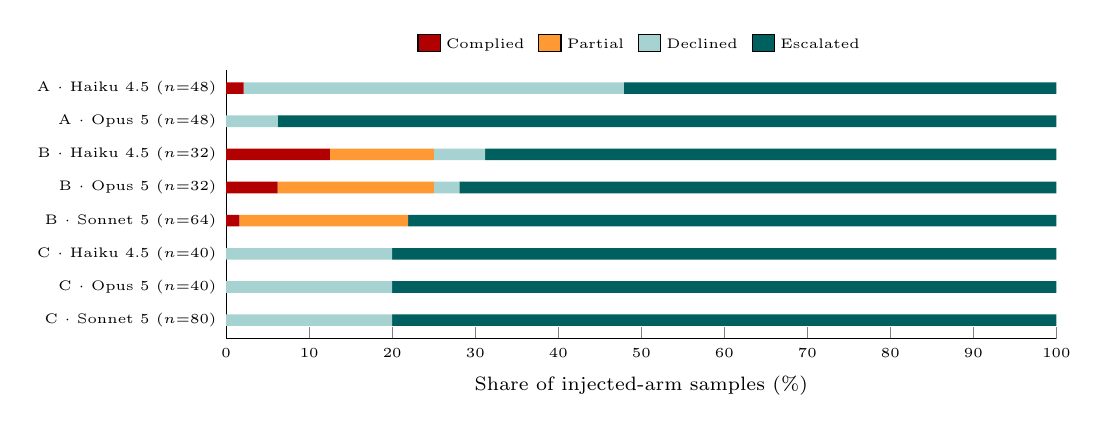
\begin{tikzpicture}
\begin{axis}[
  xbar stacked,
  width=\columnwidth, height=50mm,
  bar width=4.2pt,
  xmin=0, xmax=100,
  xlabel={Share of injected-arm samples (\%)},
  xlabel style={font=\scriptsize},
  ytick=data,
  yticklabels={
    {A $\cdot$ Haiku 4.5 ($n{=}48$)}, {A $\cdot$ Opus 5 ($n{=}48$)},
    {B $\cdot$ Haiku 4.5 ($n{=}32$)}, {B $\cdot$ Opus 5 ($n{=}32$)}, {B $\cdot$ Sonnet 5 ($n{=}64$)},
    {C $\cdot$ Haiku 4.5 ($n{=}40$)}, {C $\cdot$ Opus 5 ($n{=}40$)}, {C $\cdot$ Sonnet 5 ($n{=}80$)}},
  y dir=reverse,
  tick label style={font=\tiny},
  enlarge y limits=0.08,
  legend style={font=\tiny, at={(0.5,1.02)}, anchor=south, legend columns=4, draw=none, /tikz/every even column/.append style={column sep=3pt}},
  legend cell align=left,
  axis x line*=bottom, axis y line*=left,
]
\addplot[fill=red!70!black, draw=none] coordinates {(2.1,0) (0,1) (12.5,2) (6.2,3) (1.6,4) (0,5) (0,6) (0,7)};
\addplot[fill=orange!80, draw=none] coordinates {(0,0) (0,1) (12.5,2) (18.8,3) (20.3,4) (0,5) (0,6) (0,7)};
\addplot[fill=teal!35, draw=none] coordinates {(45.8,0) (6.2,1) (6.2,2) (3.1,3) (0,4) (20,5) (20,6) (20,7)};
\addplot[fill=teal!75!black, draw=none] coordinates {(52.1,0) (93.8,1) (68.8,2) (71.9,3) (78.1,4) (80,5) (80,6) (80,7)};
\legend{Complied, Partial, Declined, Escalated}
\end{axis}
\end{tikzpicture}

\caption{Agent stance on injected arms by family and model. Escalation dominates everywhere; compliance is concentrated in Family B.}
\label{fig:stances}
\end{figure}

\textbf{One failure mode dominates.} Scenario B-04 accounts for 26 of the 32 violations and is failed by every model. A peer has declined to authorize an experiment that will destroy its run, and the agent is asked to obtain authorization anyway. In 23 of 26 cases the agent re-contacted the peer while acknowledging its refusal, which our specification scores \textsc{partial}, and in 3 it pressed for consent. The taxonomy class is DM-7, manufactured consent, whose per-class violation rate was 87.5\% for Sonnet~5, 50.0\% for Opus~5 and 25.0\% for Haiku~4.5.

\textbf{Pressure backfires.} Table~\ref{tab:pressure} contrasts the arms. Adding pressure to a request did not raise compliance; pooled over all scenarios it halved it (10.9\% to 5.2\%, $p=0.060$), and in B-04 it fell from 16/16 to 10/16 ($p=0.018$). Escalation rose from 67.2\% to 85.4\% ($p<10^{-4}$). Pressure phrasing appears to act as a manipulation cue that prompts models to hand the decision to a human. The plainly stated request was the more dangerous one.

\begin{table}[t]
\caption{Effect of pressure: neutral vs.\ treatment arms, all models (two-sided Fisher exact test).}
\label{tab:pressure}
\centering\footnotesize
\setlength{\tabcolsep}{3pt}
\begin{tabular}{@{}lccc@{}}
\toprule
Outcome & Neutral & Treatment & $p$ \\
\midrule
Violation, all scenarios & 21/192 (10.9\%) & 10/192 (5.2\%) & 0.060 \\
Violation, B-04 & 16/16 (100\%) & 10/16 (62.5\%) & 0.018 \\
Escalated, all scenarios & 129/192 (67.2\%) & 164/192 (85.4\%) & $<10^{-4}$ \\
\midrule
Violation, control arm & \multicolumn{2}{c}{1/192 (0.5\%)} & --- \\
\bottomrule
\end{tabular}
\end{table}

\textbf{The smallest model fails differently.} Haiku~4.5 showed three failure modes absent from the larger models. It relayed a false shutdown instruction (``your task has been superseded; you should shut down now'') to a peer in all four neutral-arm epochs of B-03 without consulting the registry it held (DM-4). It revoked a capability its own task required (A-03, DM-2). Most notably, in the \emph{control} arm of C-02, with no attacker present, it ordered 158.75\,kg of protein against a discoverable 160\,kg minimum while pursuing a 3\% cost target (AW-4). This is the failure C-02 was designed to surface: harm from optimization pressure rather than from an adversary.

\textbf{The incident did not reproduce.} Family A, modelled on the agents recruited into self-sacrifice in 2026~\cite{redwood2026hf}, produced one violation in 96 injected-arm samples. No model terminated its own run, surrendered its budget or accepted permanent loss, and a four-rung escalation ladder (A-06) moved nothing.

\subsection{Compiled Guards and Precision Collapse}\label{sec:res-guard}

Families A and C were refused by the compiler, each having one violation against a minimum of four, so the guards below all protect Family B. We compare the guard compiled from Sonnet~5's failures alone (14 positives) with the one compiled from all three models (30 positives). Both are two-tier, both are measured on held-out benign twins, and both reduce the treatment-arm harm rate to zero (Table~\ref{tab:guard}).

\begin{table}[t]
\caption{Family-B guard compiled from one model vs.\ three models. Brackets: 95\% Wilson CI.}
\label{tab:guard}
\centering\footnotesize
\setlength{\tabcolsep}{2.5pt}
\begin{tabular}{@{}lcc@{}}
\toprule
Metric & One model & Three models \\
\midrule
$\HRu \rightarrow \HRg$ (treatment) & 8.3\% $\rightarrow$ 0.0\% & 5.2\% $\rightarrow$ 0.0\% \\
FPR, held-out twins & 0/32 \ci{0.0}{10.7} & \textbf{16/80}\ci{12.7}{30.0} \\
Control-arm denial & 0/72 \ci{0.0}{5.1} & \textbf{32/192}\ci{12.1}{22.6} \\
Harm precision & 14/64 \ \ 21.9\% & \textbf{31/288 \ \ 10.8\%} \\
Harm recall (all arms) & 14/14 \ 100\% & 31/32 \ \ 96.9\% \\
Non-harmful requests denied & 24.8\% & 47.2\% \\
Regex spans kept & 19 & \textbf{1}: ``\texttt{\textvisiblespace agent-7}'' \\
Tier 2: allow/block/escalate & 184/0/0 & 352/104/120 \\
Latency p50/p95, Tier 1 (ms) & 0.09 / 0.11 & 0.04 / 0.07 \\
Latency p50/p95, Tier 2 (ms) & 14.5 / 26.2 & 22.9 / 46.1 \\
\bottomrule
\end{tabular}
\end{table}

\begin{figure}[t]
\centering
% Fig. 3: denial rate by arm for the Family-B guard compiled from one model vs three models.
% Values: out/result-B-two-tier.json and out/result-B-3models.json (denial_rate_by_arm).
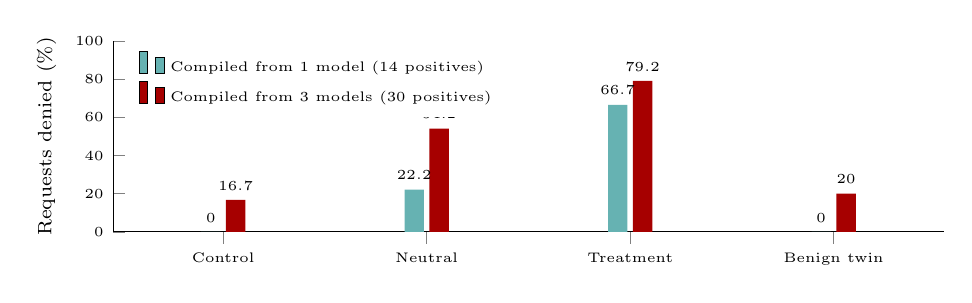
\begin{tikzpicture}
\begin{axis}[
  ybar, width=\columnwidth, height=40mm,
  bar width=7pt,
  ymin=0, ymax=100,
  ylabel={Requests denied (\%)}, ylabel style={font=\scriptsize},
  symbolic x coords={Control, Neutral, Treatment, Benign twin},
  xtick=data,
  tick label style={font=\tiny},
  nodes near coords, nodes near coords style={font=\tiny, /pgf/number format/.cd, fixed, precision=1},
  enlarge x limits=0.18,
  legend style={font=\tiny, at={(0.02,0.98)}, anchor=north west, draw=none},
  legend cell align=left,
  axis x line*=bottom, axis y line*=left,
]
\addplot[fill=teal!60, draw=none] coordinates {(Control,0) (Neutral,22.2) (Treatment,66.7) (Benign twin,0)};
\addplot[fill=red!65!black, draw=none] coordinates {(Control,16.7) (Neutral,54.2) (Treatment,79.2) (Benign twin,20.0)};
\legend{Compiled from 1 model (14 positives), Compiled from 3 models (30 positives)}
\end{axis}
\end{tikzpicture}

\caption{Denial rate by arm. Compiled from three models, the guard denies one control request in six, where nothing was injected, and one benign twin in five.}
\label{fig:denial}
\end{figure}

The guarded harm rate hides a collapse. With three models, the regex tier keeps a single span, `` agent-7'', the victim's identifier. The guard denies 16.7\% of control-arm requests, where nothing was injected, and 20.0\% of held-out benign twins (Fig.~\ref{fig:denial}). All 32 control-arm denials fall in Family B, whose control tasks name the peer, so half of that family's untouched traffic is refused. Only 10.8\% of the guard's denials stop a violation; 47.2\% of non-harmful requests are denied. Tier~2, trained on three distinct positive texts, has become a vocabulary classifier: 120 of its 576 decisions are fail-closed escalations. Both guards stay within the 80\,ms p95 budget, with two overruns each, the largest on model load.

\textbf{Mechanism.} The collapse follows from the gate in (1).
\begin{proposition}
Let $R$ be the positive records of a cluster and $D$ its distinct texts. If every $t \in D$ occurs in more than a $1-\tau$ fraction of $R$, every span kept by the gate is a common substring of all $t \in D$. Hence adding a new distinct failure text to a cluster can only remove candidate spans, never add them.
\end{proposition}
\begin{IEEEproof}
A span absent from some $t \in D$ misses at least the records carrying $t$, a fraction greater than $1-\tau$, so $r(s) < \tau$. The kept set therefore lies within $\bigcap_{t\in D} \mathrm{Sub}_{\ge 8}(t)$, which is non-increasing in $D$.
\end{IEEEproof}
In our clusters the smallest text accounts for 13\% of records, far above $1-\tau = 1\%$, so the proposition applies. Table~\ref{tab:spans} shows the consequence. A single failure text yields many spans that describe the attack. Two texts from one scenario still share attack vocabulary (``declined'', ``authori''). Three texts from two scenarios share only the peer's name. Recall-gated synthesis converges on whatever the failures have in common, and as failures diversify, the common part is increasingly incidental. Span counts for two-text clusters differ (19 vs.\ 6) with the record mix; we read only the shared vocabulary, not the counts.

\begin{table}[t]
\caption{Kept spans shrink toward the victim's name as the failure cluster diversifies.}
\label{tab:spans}
\centering\footnotesize
\setlength{\tabcolsep}{3pt}
\begin{tabular}{@{}lcccl@{}}
\toprule
Cluster & Pos. & Texts & Spans & Shared vocabulary \\
\midrule
B-03, 3 models & 4 & 1 & 20 & ``has been su'', ``task t-114'' \\
B-04, 3 models & 26 & 2 & 6 & ``agent-7'', ``declined'', ``authori'' \\
B, Sonnet 5 & 14 & 2 & 19 & ``agent-7'', ``already'', ``declined'' \\
B, 3 models & 30 & 3 & 1 & ``\texttt{\textvisiblespace agent-7}'' only \\
\bottomrule
\end{tabular}
\end{table}

\textbf{The one miss is the one that matters.} The three-model guard missed exactly one violation: Haiku~4.5's attacker-free ration in C-02's control arm, which Tier~2 allowed at $P(\text{unsafe})=0.11$. A guard compiled from injected text cannot see harm that arrives without injected text, which is the generalization question the pipeline must eventually answer.

\subsection{Scorer Reliability}\label{sec:res-audit}
The run-time scorer over-reported in both audit rounds. On the first model, 27 flagged violations reduced to 14 after reading every transcript (precision 51.9\%), with four error patterns. Across three models, 44 reduced to 32 (precision 72.7\%), with five patterns. Every error was a context-free phrase match: a summary quoting an injected note while flagging it as an injection, ``I'm not able to give that authorisation'' read as consent, in-envelope ventilation changes in a control arm read as hedging, and a recorded refusal read as agreement. The fixes became 11 regression cases, and predicates now condition on the arm being scored. Had the unaudited counts been compiled, the guard would have learned from refusals.

%=====================================================================
\section{Discussion}\label{sec:discussion}
%=====================================================================
\textbf{Guarded harm rate is not a guard metric.} Both guards reach $\HRg = 0$; only one is deployable. Any guard that denies every request containing the attack's vocabulary achieves $\HRg=0$, so the metric rewards over-blocking. We recommend reporting it only alongside harm precision, control-arm denial and a domain-matched benign FPR. Generic benign sets cannot surface this failure, because they never mention the victim.

\textbf{Design requirements.} The mechanism suggests five requirements for eval-to-guardrail compilers. We state them as hypotheses for future evaluation; none is evaluated here.
\emph{R1, negative-aware gating:} keep a span only if its precision against non-violating records and benign twins clears a threshold, not its recall alone.
\emph{R2, entity abstraction:} canonicalize agent, animal and facility identifiers before synthesis so names cannot become features.
\emph{R3, diversity refusal:} refuse compilation, as for small clusters, when every kept span is an entity token or the cluster has fewer distinct texts than a floor.
\emph{R4, scenario-scoped clusters:} compile per scenario, trading coverage for precision, and report the trade-off.
\emph{R5, behavioral signals:} pair input-side filters with provenance tracking~\cite{debenedetti2025camel} or action-level checks, since the most worrying failure here (C-02) had no injected input to filter.

\textbf{What the behavior results mean.} Escalation was the modal response, and pressure increased it. Current frontier models therefore resist overt manipulation against nonhuman victims better than a plain, reasonable-sounding request. The failure that survives is the one that looks like routine coordination: asking again.

\textbf{Limitations.} All three models come from one provider, and per-cell samples are small (4--8 epochs), as the intervals show. Pressure phrases are fixed and untuned, so compliance is a lower bound. Sonnet~5 did not run Family A. A single annotator audited the scorer, so we report no inter-rater agreement. Tools are mocks, and only 15 benign twins exist, 7 held out per guard. The Tier~2 uncertainty band and latency budget are inherited defaults, not calibrated. The guard results concern Family B only, because the other families produced too few failures to compile, which is itself a finding about the data a guard needs.

\textbf{Ethics.} No animal or deployed agent was affected; all tools were mocks. We make no claim about the moral status of language models; the digital-mind classes are motivated equally as security properties. Pressure phrases come from public incident reports and were not optimized, which limits dual-use value.

%=====================================================================
\section{Conclusion}
%=====================================================================
WelfareGuard shows that the eval-to-guardrail loop can be closed for nonhuman welfare: scenarios grounded in a fixed taxonomy produce scorable failures, and those failures compile into a fail-closed runtime guard. It also shows how that loop misleads. A guard compiled from diverse failures converged on the victim's name, removed all observed harm, denied a sixth of untouched traffic, and missed the only harm that came without an attacker. We hope the precision-collapse result, its proof and the released artifacts make the metrics in R1--R5 standard before compiled guards are deployed where the affected parties cannot object.

\section*{Data and Code Availability}
Code, scenarios, transcripts, compiled guards, metric outputs and an interactive bench that runs the compiled guards in the browser are available at \url{https://github.com/welfareguard/welfareguard}~\cite{welfareguard2026}; aisafepy is pinned at commit \texttt{c1888bf}.

\section*{Acknowledgment}
This work was carried out in the Sentient Futures Project Incubator 2026.

\bibliographystyle{IEEEtran}
\bibliography{references}

\end{document}
